\chapter{Algebraic Topology}\label{chapter:algtop}

    References for this chapter are \cite{massey, merry_io}.

\section{Homotopy theory}\label{section:homotopy}
\subsection{Homotopy}

    \newdef{Retraction}{\index{retract}
        Let $X$ be a topological space and let $A\subset X$ be a subspace. A continuous function $f:X\rightarrow A$ is called a retraction (and $A$ is called a \textbf{retract} of $X$) if it satisfies $f(a)=a$ for all $a\in A$.\footnote{It is a retraction of the inclusion map $A\hookrightarrow X$ in the sense of Definition \ref{cat:retract}.}
    }
    \newdef{Homotopy}{\index{homotopy}\label{topology:homotopy}
        Let $f,g\in C(X,Y)$ where $X,Y$ are topological spaces. If there exists a continuous function $H:X\times[0,1]\rightarrow Y$ such that $f(x) = H(x,0)$ and $g(x) = H(x,1)$, then $f$ and $g$ are said to be homotopic. This relation induces an equivalence relation on $C(X,Y)$ for which the quotient space is denoted by $[X,Y]$.
    }
    \newdef{Deformation retraction}{
        Let $X$ be a topological space and let $A\subseteq X$ be a subspace. $A$ is called a deformation retract if there exists a homotopy between the identity function on $X$ and a retraction $f:X\rightarrow A$.
    }

    \newdef{Homotopy type}{\index{homotopy!type}
        Two topological spaces $X$ and $Y$ are said to be \textbf{homotopy equivalent} or to be of the same homotopy type\footnote{The associated equivalence classes are sometimes called \textbf{strong homotopy types} to distinguish them from the homotopy types associated to the weak equivalences introduced further on.} if there exist continuous functions $f:X\rightarrow Y$ and $g:Y\rightarrow X$ such that $f\circ g$ is homotopic to $\mathbbm{1}_Y$ and $g\circ f$ is homotopic to $\mathbbm{1}_X$. The maps $f,g$ are called \textbf{homotopy equivalences}.
    }
    \begin{property}[Homeomorphisms]
        Every homeomorphism is a homotopy equivalence.
    \end{property}

    \newdef{Null-homotopic}{
        A continuous function is said to be null-homotopic if it is homotopic to a constant function.
    }
    \newdef{Contractible space}{\index{contractible}\label{topology:contractible_space}
        A topological space $X$ is said to be contractible if the identity map $\mathbbm{1}_X$ is null-homotopic or, equivalently, if the space is homotopy-equivalent to a point.
    }

    \newdef{Good cover}{\index{cover}\label{topology:good_cover}
        Let $X$ be a topological space with an open cover $\mathcal{U}=\{U_i\}_{i\in I}$. The cover $\mathcal{U}$ is called a good cover (or \textbf{nice cover}) if every nonempty finite intersection $U_{i_1}\cap\ldots\cap\,U_{i_k}$ is contractible.
    }

    \newprop{Path space}{\index{mapping!space}\label{topology:path_space}
        Consider a topological space $X$. By Property \ref{topology:internal_hom} functions $Y\rightarrow X^{[0,1]}$ to the path space represent functions $Y\times[0,1]\rightarrow X$, i.e. the path space represents homotopies to $X$.
    }

\subsection{Homotopy groups}

    In this subsection it will always be assumed that the spaces are pointed \ref{topology:pointed_space}. The generic base point will be denoted by $\ast$.

    \newdef{Loop space}{\index{loop!space}
        \nomenclature[S_zsymOmega]{$\Omega X$}{(based) loop space on $X$}
        \nomenclature[S_LX]{$LX$}{free loop space on $X$}
        The set of all \textbf{loops} in a pointed topological space $(X,\ast)$, i.e. all continuous functions $\delta:(S^1,t_0)\rightarrow (X,\ast)$ for which $\delta(t_0)=\ast$. This space is denoted by $\Omega X$. It can be turned into a topological space by equipping it with the \textit{compact-open topology}.

        When one drops the requirement of based loops, i.e. when one considers the space of all continuous functions $S^1\rightarrow X$, the resulting space is called the \textbf{free loop space} on $X$. This space is denoted by $LX$.
    }
    \newdef{Loop group}{\index{loop!group}\label{topology:loop_group}
        In the case of topological groups one can define a group structure on the (free) loop space. With the \textit{compact-open topology} it even becomes a topological group.
    }
    \begin{remark}[\difficult{$H$-structure}]\index{H-space}\label{topology:h_structure}
        Loop spaces can be equipped with a multiplication corresponding to the concatenation of loops\footnote{It should be noted that the rate at which the concatenated loops are traversed is doubled because the parameter $t$ should remain an element of $S^1\cong[0, 1]/_{0\sim1}$.}. However, this operation is not strictly associative and, hence, it does not endow the loop space with a group structure. Instead it turns the loop space into an \textit{H-group} (which is in particular an $A_\infty$-space \ref{cat:A_infinity_space}), i.e. a group up to homotopy.
    \end{remark}

    \newdef{Fundamental group}{\index{group!fundamental}
        The fundamental group $\pi_1(X,x_0)$ is defined as the loop space of $(X,x_0)$ modulo homotopy, i.e. $\pi_1(X):=\pi_0(\Omega X)$ where $\pi_0$ denotes the set of path components \ref{topology:connected_components}. As the name implies, the fundamental group can be given the structure of a multiplicative group where the operation is inherited from that of the loop space.
    }
    \begin{remark}
        In general, as the notation implies, the fundamental group depends on the base point $x_0$. However, when the space $X$ is path-connected, the fundamental groups belonging to different base points are isomorphic. It follows that one can speak of ``the'' fundamental group in the case of path-connected spaces.
    \end{remark}

    \begin{property}[Groups]\label{topology:abelian_fundamental_group}
        The fundamental group of a topological group is Abelian. This follows from an Eckmann-Hilton argument \ref{algebra:eckmann_hilton}.
    \end{property}

    \newdef{Fundamental groupoid $\clubsuit$}{\index{groupoid!fundamental}\index{Poincar\'e!groupoid}\label{topology:fundamental_groupoid}
        Let $X$ be a topological space. The fundamental (or \textbf{Poincar\'e}) groupoid $\mathbf{\Pi}_1(X)$ is the groupoid consisting of the following data:
        \begin{itemize}
            \item\textbf{Objects}: $X$
            \item\textbf{Morphisms}: The endpoint-preserving homotopy classes of continuous functions $f:S^1\rightarrow X$.
        \end{itemize}
        The fundamental group $\pi_1(X,x)$ can be recovered as the automorphism group of $x\in\text{ob}(\mathbf{\Pi}_1(X))$.
    }

    \newdef{Simply-connected space}{\index{simply-connected}\label{topology:simply_connected}
        A topological space is said to be simply-connected if it is path-connected and if the fundamental group is trivial.
    }

    \newdef{Universal covering space}{
        A covering space \ref{topology:covering_space} is said to be universal if it is simply-connected.
    }
    \begin{uproperty}
        Let $X$ be a topological space and let $\widetilde{X}$ be its the universal covering space. Every other covering space $C$ of $X$ is also covered by $\widetilde{X}$.
    \end{uproperty}
    \begin{property}[Universal cover]\index{deck transformation}
        Consider a topological space $X$ and let $\widetilde{X}$ be its universal covering space. The group of deck transformations $\text{Aut}(\widetilde{X})$ from Definition \ref{topology:deck_transformation} is isomorphic to the fundamental group $\pi_1(X)$. Hence one obtains
        \begin{gather}
            X\cong\widetilde{X}/\pi_1(X).
        \end{gather}
    \end{property}

    The definition of fundamental groups can be generalized to arbitrary dimensions. (Note that in the following definition the interval $[0,1]$ is replaced by the sphere $S^1$. This is nonrestrictive as one can construct $S^n$ by identifying the boundary of $[0,1]^n$ with the basepoint $x_0$.)
    \newdef{Homotopy group}{\index{homotopy!group}
        \nomenclature[S_zsymhos]{$\pi_n(X,x_0)$}{$n^{th}$ homotopy space over $X$ with basepoint $x_0$}
        The homotopy group $\pi_n(X,x_0)$ is defined as the set of homotopy classes of continuous functions $f:S^n\rightarrow X$ based at $x_0\in X$. The set $\pi_0(X,x_0)$ can be seen to be the set of path-connected components of $X$ (Remark \ref{topology:connected_components}). This explains why the notation $\pi_0(X)$ was introduced before.
    }
    \begin{property}\label{topology:abelian_homotopy_groups}
        For $n\geq1$ the sets $\pi_n(X,x_0)$ are groups. For $n\geq2$  the homotopy groups $\pi_n(X,x_0)$ are Abelian. This follows from an Eckmann-Hilton argument \ref{algebra:eckmann_hilton}.
    \end{property}

    \begin{property}[Path-connectedness]
        If $X$ is path-connected, the homotopy groups for different basepoints are isomorphic.
    \end{property}
    \begin{property}[Homeomorphisms]\label{topology:homeomorphic_homotopy}
        Homeomorphic spaces have isomorphic homotopy groups.
    \end{property}

    \begin{formula}[Products]
        Let $(X,x_0)$ and $(Y,y_0)$ be pointed topological spaces with homotopy groups $\pi_n(X,x_0)$ and $\pi_n(Y,y_0)$. The homotopy groups of their product is given by
        \begin{gather}
            \pi_n(X\times Y,(x_0,y_0)) = \pi_n(X,x_0)\times\pi_n(Y,y_0).
        \end{gather}
    \end{formula}

    \begin{property}[\difficult{Whitehead bracket}]
        Consider a simply-connected topological space $X$. The complex $\bigoplus_{n=1}\pi_n(X)$ obtains the structure of a graded Lie algebra when equipped with the \textit{Whitehead bracket}.
    \end{property}

    \newdef{Weak homotopy equivalence}{\index{weak!equivalence}\index{homotopy!type}\label{topology:weak_equivalence}
        A continuous function that induces isomorphisms on all homotopy groups. Two spaces connected via a weak homotopy equivalence are said to have the same \textbf{homotopy type}.
    }

    \newdef{$n$-connected space}{\index{connected}
        A topological space is said to be $n$-connected if it is path-connected and if its first $n$ homotopy groups are trivial. A continuous function is said to be $n$-connected if its induced maps on homotopy groups are isomorphisms in degrees $k<n$ and surjective in degree $n$.
    }
    \newdef{Homotopy $n$-type}{\index{homotopy!type}
        A topological space for which the homotopy groups $\pi_i$ vanish for $i>n$.
    }

    \newdef{Eilenberg-MacLane space}{\index{Eilenberg-MacLane space}\label{topology:eilenberg_maclane}
        Let $G$ be a group (regarded as a discrete topological space) and choose a positive integer $n\in\mathbb{N}_0$. An Eilenberg-MacLane space $K(G,n)$ is a topological space with the following property:
        \begin{gather}
            \pi_i\Big(K(G,n)\Big)=\begin{cases}
                G&i=n\\
                0&i\neq n.
            \end{cases}
        \end{gather}
        It follows from Property \ref{topology:abelian_homotopy_groups} above that for $n>1$ the group $G$ has to be Abelian.
    }
    \begin{property}[Uniqueness]
        For every group $G$ and integer $n\in\mathbb{N}_0$, the space $K(G,n)$ is unique up to weak homotopy equivalences.
    \end{property}
    \begin{property}[Loop spaces]
        For all groups $G$ and integers $n\geq2$, the loop space $\Omega K(G,n)$ is homotopy equivalent to $K(G,n-1)$.
    \end{property}

    \newdef{Postnikov tower\footnotemark}{\index{Postnikov tower}\index{Whitehead!tower}
        \footnotetext{Often called the \textbf{Moore-Postnikov tower} or \textbf{Postnikov system} (especially in category theory).}
        Consider a path-connected topological space $X$. A Postnikov tower of $X$ is an inverse system of topological spaces $(X_i, \phi_i)$ with the following properties:
        \begin{enumerate}
            \item for all $i\leq n$ there exists an isomorphism $\pi_i(X)\cong\pi_i(X^n)$, and
            \item for all $n$ the space $X^n$ is a homotopy $n$-type.
        \end{enumerate}
        In some cases the morphisms $\phi:X_i\rightarrow X_{i-1}$ in the inverse system are required to be fibrations (this also implies that the fibres are Eilenberg-MacLane spaces).

        The (categorically) dual notion is called the \textbf{Whitehead tower} of $X$. This consists of a sequence of topological spaces
        \begin{gather}
            \cdots\longrightarrow X_2\longrightarrow X_1\longrightarrow X
        \end{gather}
        such that:
        \begin{enumerate}
            \item for all $i>n$ the induced maps $\pi_i(X_n)\rightarrow\pi_i(X)$ are isomorphisms, and
            \item for all $n$ the space $X_n$ is $n$-connected.
        \end{enumerate}
        Again one can add the requirement that the maps $\phi_i:X_i\rightarrow X_{i-1}$ are fibrations.
    }

    The following conjecture is due to \textit{Baez}. Proofs are available depending on which model is used for the definition of $\infty$-groupoids.
    \begin{theorem}[\difficult{Homotopy hypothesis}]\index{homotopy hypothesis}
        $\mathbf{Top}$ and $\mathbf{\infty Grpd}$ are equivalent as $(\infty, 1)$-categories. In particular this means that $n$-groupoids are equivalent to homotopy $n$-types.
    \end{theorem}
    \begin{remark}
        The statement of the above theorem is sometimes used as a consistency condition for the definition of $\infty$-categories and in some cases it is even used as the very definition of higher groupoids. It should also be noted that the relation is very important in homotopy type theory as introduced in Chapter \ref{chapter:type_theory}.
    \end{remark}

    \begin{property}[Homotopy category $\clubsuit$]
        \nomenclature[S_hTop]{\textbf{hTop}}{Homotopy category}
        The homotopy category $\mathbf{hTop}$ has as objects the topological spaces and as morphisms the homotopy classes of continuous functions. It is immediately clear that there exists a functor $F:\mathbf{Top}\rightarrow\mathbf{hTop}$ that acts as the identity on spaces and maps continuous functions to their homotopy classes.

        However, the above definition is often too restrictive. \textit{Quillen} gave a more general construction. The homotopy category (in the sense of Quillen) is obtained as the localization \ref{cat:localization} of $\mathbf{Top}$ with respect to the collection of weak homotopy equivalences. (See Section \ref{section:model_categories} for more information.)
    \end{property}

    Recall the reduced suspension functor $\Sigma$ from Definition \ref{topology:suspension}. The functors $\Sigma$ and $\Omega$ are related in the following way:
    \begin{property}[Eckmann-Hilton duality]\index{Eckmann-Hilton duality}\label{topology:eckmann_hilton}
        The reduced suspension functor $\Sigma$ and the loop space functor $\Omega$ form an adjunction in the category of pointed topological spaces:
        \begin{gather}
            \text{Map}_*(\Sigma X,Y)\cong\text{Map}_*(X,\Omega Y).
        \end{gather}
        This also passes down to an equivalence in the associated homotopy category:
        \begin{gather}
            [\Sigma X,Y]\cong[X,\Omega Y].
        \end{gather}
    \end{property}
    \begin{result}
        By choosing $X=S^n$ and using the result from Example \ref{topology:sphere_suspension}, one obtains the following important result for homotopy groups:
        \begin{gather}
            \pi_{n+1}(Y)\cong\pi_n(\Omega Y).
        \end{gather}
    \end{result}

    \begin{theorem}[Freudenthal suspension theorem]\index{Freudenthal suspension theorem}\label{topology:freudenthal}
        The suspension morphism in homotopy
        \begin{gather}
            \pi_{n+k}(S^n)\rightarrow\pi_{n+k+1}(S^{n+1})
        \end{gather}
        is an isomorphism for all $k\leq n-2$.
    \end{theorem}

\subsection{CW complexes}

    \newdef{$n$-cell}{\index{cell}
        An open $n$-cell is a subset of a topological space homeomorphic to an $n$-dimensional open ball. A closed $n$-cell is the image of an $n$-dimensional closed ball under an attaching map \ref{topology:attaching_space}.
    }

    \newdef{CW complex}{\index{CW!complex}\label{topology:cw_complex}
        A CW complex is a Hausdorff space $X$ together with a partition of $X$ in open cells satisfying following conditions:
        \begin{enumerate}
            \item A subset of $X$ is closed if and only if it intersects the closure of each cell in a closed set.
            \item For each open $n$-cell $C$ in the partition there exists an attaching map $f:\overline{B}_n\rightarrow X$ such that:
            \begin{itemize}
                \item $f|_{B_n}$ is homeomorphic to $C$, and
                \item $f(\partial\overline{B}_n)$ is covered by a finite number of open cells in the partition, each having dimension smaller than $n$.
            \end{itemize}
        \end{enumerate}
    }
    \newdef{Regular CW complex}{
        A CW complex such that for every open cell $C$ the attaching map $f$ is a homeomorphism onto the closure $\overline{C}$.
    }
    \newdef{Finite type}{\index{finite!type}
        A CW complex is said to be of finite type if there are only a finite number of cells in each degree.
    }

    \begin{construct}\index{skeleton}
        Every CW complex can be constructed inductively (up to isomorphism):
        \begin{quote}
            First, choose a discrete space $X_0$. This space forms the collection of 0-cells. Then, one adds 1-cells $C_1$ using appropriate attaching maps $f:\partial\overline{B}_1\rightarrow X_0$. This way a 1-dimensional CW complex $X_1$ is obtained. Inductively one obtains a sequence of nested $n$-dimensional CW complexes $X_0\subset X_1\subset\cdots\subset X_n$.
        \end{quote}
        The spaces $X_i$ are also called \textbf{$i$-skeletons}.
    \end{construct}
    \remark{Infinite-dimensional CW complexes can be obtained by taking the direct limit \ref{algebra:direct_limit} of the sequence above.}

    \begin{theorem}[Whitehead]\index{Whitehead}\label{topology:whitehead}
        A continuous function between CW complexes is a homotopy equivalence if and only if it is a weak homotopy equivalence.
    \end{theorem}
    \begin{theorem}[CW approximation theorem]\index{CW!approximation theorem}
        For every topological space $X$ there exists a CW complex $Y$ together with a weak homotopy equivalence $f:X\rightarrow Y$.
    \end{theorem}

    \begin{property}[Suspensions]
        The suspension and reduced suspension of a CW complex are weakly homotopy equivalent.
    \end{property}

    Because the unit $X\rightarrow\Omega\Sigma X$ of the Eckmann-Hilton adjunction is $(2n+1)$-connected, the Freudenthal suspension theorem \ref{topology:freudenthal} can be generalized to CW complexes:
    \begin{theorem}[Freudenthal suspension theorem]\index{Freudenthal suspension theorem}
        If $X$ is $n$-connected, the suspension morphism
        \begin{gather}
            \pi_k(X)\rightarrow\pi_{k+1}(\Sigma X)
        \end{gather}
        is an isomorphism for all $k\leq2n$.
    \end{theorem}

\subsection{Fibrations}

    \newdef{Homotopy lifting property}{
        Consider a continuous function $\pi:E\rightarrow B$. This function is said to have the homotopy lifting property with respect to a topological space $X$ if for every homotopy $f:X\times[0, 1]\rightarrow B$ and lift $\widetilde{f}_0:X\rightarrow E$ of $f_0:=f|_{X\times\{0\}}$ there exists a homotopy $\widetilde{f}:X\times[0, 1]$ lifting $f$ such that diagram \ref{fig:homotopy_lifting_property} commutes.

        \begin{figure}[ht!]
            \centering
            \begin{tikzpicture}
                \node (X) at (0,0) {$X$};
                \node (E) at (4,0) {$E$};
                \node (XI) at (0,-2) {$X\times [0,1]$};
                \node (B) at (4,-2) {$B$};
                \draw[->] (X) -- node[above]{$\widetilde{f}_0$} (E);
                \draw[right hook ->] (X) -- node[left]{$X\times\{0\}$} (XI);
                \draw[->] (XI) -- node[below]{$f$} (B);
                \draw[->] (E) -- node[right]{$\pi$} (B);
                \draw[dashed, ->] (XI) -- node[above left]{$\widetilde{f}$} (E);
            \end{tikzpicture}
            \caption{Homotopy lifting property.}
            \label{fig:homotopy_lifting_property}
        \end{figure}
    }

    \newdef{Fibration}{\index{fibration}\index{Hurewicz|seealso{fibration}}\index{Serre|seealso{fibration}}\label{topology:fibration}
        A continuous function satisfying the homotopy lifting property with respect to every topological space is called a \textbf{Hurewicz fibration}. If the homotopy lifting property only holds with respect to CW complexes, it is called a \textbf{Serre fibration}.
    }
    \begin{property}[Model fibre]
        Consider a fibration $\pi:E\rightarrow B$ with $B$ path-connected. All fibres, i.e. sets $\pi^{-1}(\{b\})$ with $b\in B$, are homotopy-equivalent. Therefore a fibration is often denoted by the diagram $\prin{F}{E}{B}$.
    \end{property}

    \begin{example}[Hopf fibration]\index{Hopf!fibration}\index{Adam}
        The Hopf fibration is given by
        \begin{gather}
            \prin{S^1}{S^3}{S^2}.
        \end{gather}
        \textit{Adam's theorem} states that this fibration can be generalized to other dimensions as $\prin{S^n}{S^{2n+1}}{S^{2n}}$ only for $n\in\{0,1,3,7\}$. (It is not a coincidence that these dimensions correspond to the dimensions of Euclidean spaces where one can consistently define a cross product or the dimensions of the real division algebras as classified by the Hurwitz theorem \ref{linalgebra:hurwitz})
    \end{example}
    \begin{example}
        For all $n\in\mathbb{N}$ the following sequence forms a fibration:
        \begin{gather}
            \prin{\text{SO}(n)}{\text{SO}(n+1)}{S^n}.
        \end{gather}
    \end{example}

    \newdef{Homotopy extension property}{
        Consider a continuous function $\iota:A\rightarrow X$. This function is said to have the homotopy extension property with respect to a topological space $Y$ if for every homotopy $f:A\times[0,1]\rightarrow Y$ and extension $\widetilde{f}_0:X\rightarrow Y$ of $f_0:=f|_{A\times\{0\}}$ there exists a homotopy $\widetilde{f}:X\times[0,1]\rightarrow Y$ extending $f$ such that diagram \ref{fig:homotopy_extension_property} (where Property \ref{topology:internal_hom} is used to represent homotopies in terms of the path space of $Y$).

        \begin{figure}[ht!]
            \centering
            \begin{tikzpicture}
                \node (Y) at (0,0) {$Y$};
                \node (X) at (4,0) {$X$};
                \node (YI) at (0,-2) {$Y^{[0,1]}$};
                \node (A) at (4,-2) {$A$};
                \draw[->] (X) -- node[above]{$\widetilde{f}_0$} (Y);
                \draw[->>] (YI) -- node[left]{$\pi_0$} (Y);
                \draw[->] (A) -- node[below]{$f$} (YI);
                \draw[->] (A) -- node[right]{$\iota$} (X);
                \draw[dashed, ->] (X) -- node[above left]{$\widetilde{f}$} (YI);
            \end{tikzpicture}
            \caption{Homotopy extension property.}
            \label{fig:homotopy_extension_property}
        \end{figure}
    }
    \newdef{Cofibration}{\index{cofibration}\label{topology:cofibration}
        A continuous function $\iota:A\rightarrow X$ satifying the homotopy extension property with respect to every topological space $Y$, i.e. every extension along $\iota$ induces an extension of homotopies or, equivalently, the extensions $C(A,Y)\rightarrow C(X,Y)$ pass down to extensions $[A,Y]\rightarrow[X,Y]$.
    }

    \begin{construct}[Mapping path space]\index{mapping!path space}\index{mapping!fibre}\index{homotopy!fibre|see{mapping fibre}}\label{topology:mapping_path_space}
        Consider a continuous function $f:X\rightarrow Y$. The mapping path space $P_f$ is defined as the following pullback:
        \begin{gather}
            P_f := \big\{(x,p)\in X\times Y^{[0,1]}\,\big\vert\,f(x)=p(0)\big\}.
        \end{gather}
        The projection
        \begin{gather}
            \pi:P_f\rightarrow Y:(x,p)\mapsto p(1)
        \end{gather}
        is a fibration. The homotopy type of the fibres of this fibration is called the \textbf{homotopy fibre} or \textbf{mapping fibre} of $f$.
    \end{construct}

    \begin{construct}[Mapping cylinder]\index{mapping!cylinder}\index{mapping!cone}\label{topology:mapping_cylinder}
        Let $f:X\rightarrow Y$ be a continuous function. The mapping cylinder $M_f$ or $\mathrm{Cyl}(f)$ is defined as follows:
        \begin{gather}
            M_f := \left(X\times[0,1]\bigsqcup Y\right)/\sim_f,
        \end{gather}
        where the equivalence relation $\sim_f$ is generated by the relations $(0,x)\sim f(x)$. So the mapping cylinder of $f:X\rightarrow Y$ is the attaching space $(X\times[0,1])\cup_f Y$. From this definition it follows that the ``top'' of the cylinder is homeomorphic to $X$ and the ``base'' is homeomorphic to $f(X)\subseteq Y$.

        By also quotienting out the relation $(1,x)\sim(1,x')$, i.e. by collapsing the top of the cylinder to a point, one obtains the so-called \textbf{mapping cone} $C_f$ or $\mathrm{Cone}(f)$. The canonical map $\iota:Y\rightarrow C_f$ is a cofibration for all continuous functions $f:X\rightarrow Y$. Furthermore, if the image $\iota(Y)$ is closed, the coprojection $C_f\rightarrow Y/f(X)$ is a homotopy equivalence.
    \end{construct}
    \begin{remark}[\difficult{Pushouts}]
        Just like the attaching space \ref{topology:attaching_space} could be obtained as a pushout in $\mathbf{Top}$, one can also characterize the mapping cone as a pushout. The cone $\mathrm{Cone}(X)$ can be obtained as the pushout of the span $\{\ast\}\leftarrow X\overset{\iota_0}{\rightarrow}X\times[0,1]$. The mapping cone is then obtained as the pushout of the span $\mathrm{Cone}(X)\leftarrow X\times[0,1]\rightarrow M_f$. By the \textit{pasting law} for pushouts this implies that the mapping cone of $f$ can be obtained as the pushout
        \begin{gather*}
            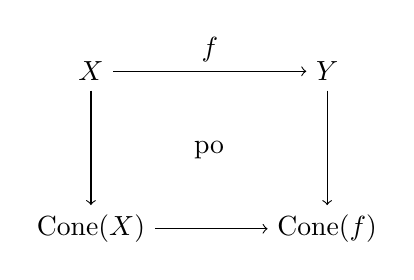
\begin{tikzpicture}
                \node (X) at (0, 0) {$X$};
                \node (Y) at (3, 0) {$Y$};
                \node (coneX) at (0, -2) {$\mathrm{Cone}(X)$};
                \node (conef) at (3, -2) {$\mathrm{Cone}(f)$};
                \node at (1.5, -1) {po};
                \draw[->] (X) -- node[above]{$f$} (Y);
                \draw[->] (X) -- (coneX);
                \draw[->] (Y) -- (conef);
                \draw[->] (coneX) -- (conef);
            \end{tikzpicture}
        \end{gather*}
    \end{remark}

\subsection{\difficult{Rational homotopy theory}}

    For the theory on differential graded algebras, see Chapter \ref{chapter:hda}.

    \newdef{Rational space}{\index{rational!space}
        A simply connected topological space $X$ for which the homotopy groups $\pi_n(X)$ are rational vector spaces.
    }

    \newdef{Rational homotopy equivalence}{\index{rational!homotopy equivalence}
        A continuous function $f:X\rightarrow Y$ for which the induced maps on rational homotopy groups
        \begin{gather}
            \pi_n(f)\otimes\mathbb{Q}:\pi_n(X)\otimes\mathbb{Q}\rightarrow\pi_n(Y)\otimes\mathbb{Q}
        \end{gather}
        are isomorphisms for all $n\in\mathbb{N}$. An equivalent requirement is that the induced map on rational (co)homology is an isomorphism (see the section on singular homology below).
    }

    \newdef{Rational homotopy category}{
        Consider the category \textbf{Top} of topological spaces. The rational homotopy category is obtained as the localization \ref{model:localization} of \textbf{Top} with respect to the collection of rational homotopy equivalences.
    }

    \newdef{Polynomial differential forms}{
        Consider the standard $n$-simplex $\Delta^n$ (Definition \ref{topology:simplex}). On this topological space one can define differential forms analogous to those from Section \ref{section:forms}. Let $\{t_i\}_{0\leq i\leq n}$ be $n+1$ generators in degree 0 (the barycentric coordinates). Together with $n+1$ associated generators $dt_i$ in degree 1, one can construct the free GCA over $\mathbb{Q}$. To preserve the geometric structure of $\Delta^n$ one has to quotient out the following relations:
        \begin{gather}
            \sum_{i=0}^n t_i = 1\qquad\text{and}\qquad\sum_{i=0}^n dt_i = 0.
        \end{gather}
        The resulting graded algebra is denoted by $\Omega^\bullet_{\text{poly}}(\Delta^n)$. In degree 0 this complex can be identified with the space of polynomial functions on $\Delta^n$. The ordinary differential forms can be obtained by taking the tensor product of $\Omega^\bullet_{\text{poly}}$ with the space of smooth functions on $\Delta^n$. Under this isomorphism the generators $dt_i$ are identified with the de Rham differentials of the barycentric coordinates.

        Morphisms $f:[m]\rightarrow[n]$ in the simplex category $\Delta$ induce morphisms of simplices and these in turn induce morphisms $F:\Omega^\bullet_{\text{poly}}(\Delta^n)\rightarrow\Omega^\bullet_{\text{poly}}(\Delta^m)$ defined by the following action on generators:
        \begin{gather}
            F(t_i) := \sum_{f(j)=i}t_j.
        \end{gather}
        It can be seen that this turns the above construction into a functor $\func{\Omega^\bullet_{\text{poly}}}{\Delta^{op}}{dgcAlg}$. By passing to the opposite functor and taking a left Kan extension along the Yoneda embedding $\Delta\hookrightarrow\mathbf{sSet}$, one obtains a functor $\func{\Omega^\bullet_{\text{poly}}}{sSet}{dgcAlg^{op}}$. Composition with the singular set functor $\func{\text{Sing}}{Top}{sSet}$ gives the \textbf{piecewise-polynomial differential forms} functor $\Omega^\bullet_{\text{pwpoly}}$.
    }

    \newdef{Relative Sullivan algebra}{\index{Sullivan!algebra}\label{topology:sullivan_algebra}
        An inclusion of DGCAs of the form \[(A,d)\hookrightarrow(A\otimes\Lambda^\bullet V,d'),\] where $A$ is any DGCA and $V$ is a $\mathbb{N}_0$-graded vector space such that:
        \begin{itemize}
            \item there is a well-ordered set $I$ indexing a linear basis $\{e_i\}_{i\in I}$ of $V$.
            \item for all $k\in I$ and all $e_k$ one has that
            \begin{gather}
                d'e_k\in A\otimes\Lambda^\bullet V(<k),
            \end{gather}
            where $V(<k):=\text{span}\{e_i\}_{i<k}$.
        \end{itemize}
        If in addition the implication
        \begin{gather}
            i<j\implies\deg(e_i)\leq\deg(e_j)
        \end{gather}
        holds for all $i,j\in I$, the relative Sullivan algebra is said to be \textbf{minimal}.

        If the Sullivan algebra is defined relative to the tensor unit $(k,0)$, where $k$ is the underlying field, it is just called a \textbf{Sullivan algebra}.
    }
    \begin{remark}
        The minimality condition admits an (equivalent) reformulation:
        \begin{gather}
            dV\subseteq A_{\geq1}\otimes\Lambda^\bullet V + A\otimes\Lambda^{\geq2}V.
        \end{gather}
    \end{remark}

    \begin{example}\label{topology:sullivan_algebras_specific}
        Consider the free DGCA $\Lambda(V)$ on a graded vector space $V$ of finite type with $V_0=V_1=0$. Then $(\Lambda(V),d)$ is a Sullivan algebra.
    \end{example}

    \newdef{Sullivan model}{\index{Sullivan!model}
        Let $X$ be a simply-connected topological space. A (minimal) Sullivan model for $X$ is a (minimal) Sullivan algebra equipped with a quasi-isomorphism to the DGA of piecewise-polynomial differential forms on $X$.
    }
    \begin{property}
        Minimal Sullivan models are unique up to isomorphism.
    \end{property}

    There is also another approach due to \textit{Quillen}. Instead of working with differential graded algebras, \textit{Quillen} used differential graded Lie algebras, i.e. strict $L_\infty$-algebras (Section \ref{section:higher_lie_structures}).
    \begin{construct}[Sketch, Quillen]
        To every simply-connected topological space $X$ one can associated a differential graded Lie algebra $L_\bullet(X)$ such that the homology of this complex is isomorphic to the (shifted) rational homotopy complex $\pi_{\bullet+1}(X)\otimes\mathbb{Q}$ of $X$.
    \end{construct}

\subsection{\difficult{Equivariant homotopy theory}}

    In this section topological spaces equipped with an action of a topological group $G$ will be considered (the group will often be a compact Lie group). Some notions will be defined very similarly to those in the previous section, but some others will look very differently.

    \newnot{Fixed-point space}{\index{fixed point}
        Consider a topological $G$-space $X$. The set of all its fixed points is denoted by $X^G$.
    }

    \newdef{Equivariant homotopy equivalence}{\index{homotopy!equivalence}
        A continuous function that is both an equivariant function and a homotopy equivalence in the ordinary sense.
    }
    \newdef{Weak equivariant homotopy equivalence}{
        An equivariant continuous function that restricts to an ordinary weak equivalence between the fixed-point subspaces for all closed subgroups $H\subset G$.
    }

    \begin{theorem}[Whitehead\footnotemark]\index{Whitehead}
        \footnotetext{This equivariant version of Theorem \ref{topology:whitehead} is due to \textit{Bredon}.}
        A continuous function between $G$-CW complexes is a weak equivariant homotopy equivalence if and only if it is a equivariant homotopy equivalence.
    \end{theorem}

    \newdef{Orbit category}{
        Let $G$ be a topological group. The orbit category $\mathbf{Orb}_G$ is the category defined by the following data:
        \begin{enumerate}
            \item the coset spaces $G/H$ with $H\subset G$ a closed subgroup as objects, and
            \item the equivariant homomorphisms as morphisms.
        \end{enumerate}
    }
    \begin{theorem}[Elmendorf]\index{Elmendorf}\index{orbit!category}
        The map $(X,H)\mapsto X^H$ sending a $G$-space to its fixed-point spaces can be interpreted as a functor $X:\mathbf{Orb}_G^{op}\rightarrow\mathbf{Top}$ or, equivalently, as a $\mathbf{Top}$-valued presheaf on the orbit category. By taking this a step further, one obtains a functor sending every topological space $X$ to such a presheaf.\footnote{This is the restriction of the Yoneda embedding to the subcategory $\mathbf{Orb}_G$ of $G\mathbf{Top}$.} To study the homotopy theory on these categories, one needs a choice of weak equivalences. Similar to the model structure on $\mathbf{sSet}$, one can choose the weak equivalences on $\mathbf{Psh}(\mathbf{Orb}_G)$ to be the levelwise weak equivalences. This gives an $(\infty,1)$-equivalence
        \begin{gather}
            \mathbf{Ho}(G\mathbf{Top})\cong\mathbf{Psh}(\mathbf{Orb}_G).
        \end{gather}
    \end{theorem}

    ?? COMPLETE ??

\section{Simplicial homology}\label{section:homology}
\subsection{Simplices}

    \newdef{Simplex}{\index{simplex}\index{vertex}\label{topology:simplex}
        A $k$-simplex $\sigma^k\equiv[t_0,\ldots,t_k]$ is defined as the following set:
        \begin{gather}
            \sigma^k := \left\{\sum_{i=0}^k\lambda_it_i\,\middle\vert\,\sum_{i=0}^k\lambda_i = 1\text{ and }\lambda_i\geq0\right\}.
        \end{gather}
        where the \textbf{vertices} $t_i\in\mathbb{R}^n$ are \textbf{affinely independent}, i.e. the vectors $t_i-t_0$ are linearly independent. Equivalently, a simplicial $k$-simplex  is the convex hull of the $k+1$ vertices $\{t_0,\ldots,t_k\}$.
    }
    \begin{remark}[Barycentric coordinates]\index{barycenter}
        The numbers $\lambda_i$ from the previous definition are called barycentric coordinates. This terminology stems from the fact that the point $\sum_{i=0}^k\lambda_it_i$ represents the \textit{barycenter} of a gravitational system consisting of masses $\lambda_i$ placed at the points $t_i$.
    \end{remark}
    \begin{example}[Standard simplex]\index{simplex!standard}\label{topology:standard_simplex}
        \begin{gather}
            \Delta^k := \left\{(x_0,\ldots,x_k)\in\mathbb{R}^{k+1}\,\middle\vert\,\sum_ix_i = 1 \text{ and }x_i\geq0\right\}
        \end{gather}
    \end{example}

    \newnot{Face}{\index{face}
        Consider a $k$-simplex $[v_0,\ldots,v_k]$. The \textbf{face} opposite to the vertex $v_i$ is the $(k-1)$-simplex $[v_0,\ldots,\widehat{v}_i,\ldots,v_k]$ obtained by removing the vertex $v_i$.
    }

    \newdef{Simplicial complex}{\index{simplicial!complex}
        A simplicial complex $\mathcal{K}$ is a set of simplices satisfying the following conditions:
        \begin{itemize}
            \item If $\sigma$ is a simplex in $\mathcal{K}$, so are its faces.
            \item If $\sigma_1,\sigma_2\in\mathcal{K}$, either $\sigma_1\cap\sigma_2 = \emptyset$ or $\sigma_1\cap\sigma_2$ is a face of both $\sigma_1$ and $\sigma_2$.
        \end{itemize}
        A simplicial $k$-complex is a simplicial complex where every simplex has dimension at most $k$.
    }

    \newdef{Path-connected complex}{\index{path!connected}
        A simplicial complex is said to be path-connected if every two vertices in are connected by an edge in.
    }

    \newdef{Polyhedron}{\index{polyhedron}
        Consider a simplicial complex. The polyhedron associated with it is the topological space constructed by equipping the complex with the Euclidean subspace topology.
    }

    \newdef{Triangulable spaces}{\index{triangulation}
        Let $X$ be a topological space and let $\mathcal{K}$ be a polyhedron. If there exists a homeomorphism $\varphi:\mathcal{K}\rightarrow X$, then $X$ is said to be triangulable and $\mathcal{K}$ is called a \textbf{triangulation} of $X$.
    }
    \begin{property}[Fundamental group]
        Let $\mathcal{K}$ be a path-connected polyhedron with basepoint $a_0$ and consider a contractible one-dimensional subpolyhedron $\mathcal{C}\subset\mathcal{K}$ containing all vertices of $\mathcal{K}$. Let $G$ be the free group \ref{group:free_group} with generators $g_{ij}$ corresponding to the ordered 1-simplices $[v_i,v_j]\in\mathcal{K}$. On this group one can define the following relations:
        \begin{itemize}
            \item $g_{ij} = e$ if $[v_i,v_j]\in\mathcal{C}$.
            \item $g_{ij}g_{jk} = g_{ik}$ for every ordered 2-simplex $[v_i,v_j,v_k]\in\mathcal{K}\backslash\mathcal{C}$.
        \end{itemize}
        The quotient group of $G$ by these relations is isomorphic to the fundamental group $\pi_1(\mathcal{K},a_0)$.
    \end{property}
    \begin{result}
        Property \ref{topology:homeomorphic_homotopy}, which states that homeomorphic spaces have the same homotopy groups, implies that the fundamental group of a triangulable space can be computed by looking at its triangulations.
    \end{result}

\subsection{Simplicial homology}

    \newdef{Chain group}{\index{chain!group}\label{topology:chain_group}
        Let $\mathcal{K}$ be a simplicial $n$-complex. The $k^{th}$ chain group $C_k(\mathcal{K})$ is defined as the free Abelian group generated by the $k$-simplices in $\mathcal{K}$:
        \begin{gather}
            C_k(\mathcal{K}) := \left\{\sum_ia_i\sigma_i\,\middle\vert\,\sigma_i\text{ is a $k$-simplex in $\mathcal{K}$}, a_i\in\mathbb{Z}\right\}.
        \end{gather}
        For $k>n$ and $k<0$, $C_k(\mathcal{K})$ is defined to be $\{0\}$.
    }

    \newdef{Boundary operator}{\index{boundary}
        The boundary operator $\partial_k:C_k(\mathcal{K})\rightarrow C_{k-1}(\mathcal{K})$ is the group morphism defined by the following properties:
        \begin{itemize}
            \item\textbf{Linearity}:
                \begin{gather}
                    \partial_k\left(\sum_ia_i\sigma_i\right) = \sum_ia_i\partial_k\sigma_i,
                \end{gather}
            \item\textbf{Action on generators}
                \begin{align}
                    \partial_k[v_0,\ldots,v_k] &= \sum_{i=0}^k(-1)^i[v_0,\ldots,\hat{v}_i,\ldots,v_k],\\
                    \partial_0[v] &= 0.
                \end{align}
        \end{itemize}
    }

    \begin{property}[Chain condition]\label{topology:boundary_operator_relation}
        The boundary operators satisfy the following relation:
        \begin{gather}
            \partial_k\circ\partial_{k+1} = 0.
        \end{gather}
        This property turns the system $(C_k,\partial_k)$ into a chain complex \ref{homalg:chain_complex}.
    \end{property}

    \newdef{Cycle group}{\index{cycle}
        The $k^{th}$ cycle group $Z_k(\mathcal{K})$ is defined as the set of $k$-chains $\sigma_k$ such that $\partial_k\sigma_k = 0$. These chains are called \textbf{cycles}.
    }
    \newdef{Boundary group}{
        The $k^{th}$ boundary group $B_k(\mathcal{K})$ is defined as the set of $k$-chains $\sigma_k$ for which there exists a $(k+1)$-chain $N$ such that $\partial_{k+1}N = \sigma_k$. These chains are called \textbf{boundaries}.
    }
    \newdef{Homology group}{\index{homology!simplicial}
        From Property \ref{topology:boundary_operator_relation} it follows that $B_k(\mathcal{K})\subset Z_k(\mathcal{K})$ is a subgroup. One can thus define the $k^{th}$ homology group $H_k(\mathcal{K})$ as the following quotient group:
        \begin{gather}
            H_k(\mathcal{K}) := Z_k(\mathcal{K})/B_k(\mathcal{K}).
        \end{gather}
        Theorem \ref{group:theorem:free_group} says that $H_k(\mathcal{K})$ can be written as $G_k\oplus T_k$. Both of these groups say something about $\mathcal{K}$. The rank of $G_k$, denoted by $R_k(\mathcal{K})$, is equal to the number of $(k+1)$-dimensional holes in $\mathcal{K}$. The torsion subgroup $T_k$ says how the space $\mathcal{K}$ is ``twisted''.
    }

    \newdef{Betti numbers}{\index{Betti number}
        The ranks $R_k(\mathcal{K})$ are called the Betti numbers of $\mathcal{K}$.
    }
    \begin{definition}[Euler characteristic]\index{Euler!characteristic}\index{Euler-Poincar\'e formula}\label{topology:euler_characteristic}
        The Euler characteristic of a triangulable space $X$ is defined as follows:
        \begin{gather}
            \chi(X) := \sum_i(-1)^iR_i(X).
        \end{gather}
        This formula is sometimes called the \textbf{Poincar\'e} or \textbf{Euler-Poincar\'e} formula.
    \end{definition}

    \begin{property}[Isomorphisms]
        If two topological spaces have the same homotopy type, in particular when they are homeomorphic, they have isomorphic homology groups.
    \end{property}
    \begin{result}
        As was the case for the fundamental group, it follows from the definition of a triangulation that one can study the homology groups of a given triangulable space by looking at its triangulations.
    \end{result}

    Although the homology invariants do not depend on the choice of triangulation, a remark about the existence of nonequivalent triangulations should be given.
    \begin{remark}[Hauptvermutung $\clubsuit$]
        Before the construction of a counterexample it was believed (hence the terms \textit{Hauptvermutung} in German or \textit{main conjecture} in English) that every two triangulations of a topological space allowed a common refinement and, hence, where equivalent for many constructions. However, it was shown that this conjecture is generally false, e.g. for topological manifolds in dimensions 5 and higher there exist an infinite number of nonequivalent triangulations. In dimensions up to 4 it was proven by Rad\'o and Moise that the Hauptvermutung holds for all topological manifolds (see also Theorem \ref{diff:rado_moise}).
    \end{remark}

    \begin{construct}
        The definition of homology groups can be generalized by letting the (formal) linear combinations used in the definition of the chain group be of the following form:
        \begin{gather}
            c = \sum_ig_i\sigma_i^k,
        \end{gather}
        where $g_i\in G$ for some Abelian group $G$. The $k^{th}$ homology group of $X$ with coefficients in $G$ is denoted by $H_k(X;G)$.
    \end{construct}
    \begin{property}[Vanishing torsion]
        When $G$ is a field, such as $\mathbb{Q}$ or $\mathbb{R}$, the torsion subgroups $T_k$ vanish. The relation between integral homology and homology with coefficients in a group is given by the \textit{universal coefficient theorem}.
    \end{property}

    \newformula{K\"unneth formula}{\index{K\"unneth formula}
        Let $X,Y$ be two simplicial complexes. The homology groups of the Cartesian product $X\times Y$ with coefficients in a field $F$ is given by
        \begin{gather}
            H_k(X\times Y;F) = \bigoplus_{k=i+j}H_i(X;F)\otimes H_j(Y;F).
        \end{gather}
        When the requirement of $F$ being a field is relaxed to it merely being a group, the torsion subgroups have to be taken into account. See the literature for this general form.
    }

\subsection{Relative homology}

    In this section the homology of a simplicial complex $K$ ``modulo'' a subcomplex $L$ is considered.

    \newdef{Relative chain group}{\index{chain}
        The $k$-chain group of $K$ modulo $L$ is defined as the following quotient group:
        \begin{gather}
            C_k(K,L) := C_k(K)/C_k(L).
        \end{gather}
        Equivalence classes will be denoted by square brackets $[c]$, where $c\in C_\bullet(K)$.
    }
    \newdef{Relative boundary operator}{\index{boundary}
        The relative boundary operator $\overline\partial_k$ is defined as follows:
        \begin{gather}
            \overline\partial_k[c_k] := [\partial_kc_k],
        \end{gather}
        where $\partial_k$ on the right-hand side denotes the boundary operator in ordinary homology. This is a well-defined operation since $\partial C_\bullet(L)\subseteq C_\bullet(L)$.
    }
    \newdef{Relative homology groups}{\index{homology!relative}
        The relative cycle and relative boundary groups are defined analogous to their ordinary counterparts. The relative homology groups are defined as follows:
        \begin{gather}
            H_k(K,L) := \stylefrac{\ker(\overline\partial_k)}{\im(\overline\partial_{k+1})}.
        \end{gather}
        Elements $h_k\in H_k(K,L)$ can be represented as $h_k=z_k + C_k(L)$ such that $\partial_kz_k\in C_{k-1}(L)$.
    }

    \begin{property}[Homotopy invariance]
        Consider two topological spaces $X,Y$ with subspaces $A\subset X,B\subset Y$. If a continuous function $f:X\rightarrow Y$ is a homotopy equivalence such that the restriction to $A$ gives a homotopy equivalence $f|_A:A\rightarrow B$, the relative homology complexes $H_\bullet(X,A)$ and $H_\bullet(Y,B)$ are isomorphic.
    \end{property}

    \begin{property}[Long sequence for a pair]
        The relative homology groups fit in the following (long) exact sequence:
        \begin{gather}
            \cdots\longrightarrow H_k(L)\overset{i_\ast}{\longrightarrow}H_k(K)\overset{j_\ast}{\longrightarrow}H_k(K,L)\overset{\partial_k}{\longrightarrow}H_{k-1}(L)\longrightarrow\cdots,
        \end{gather}
        where $i_\ast$ and $j_\ast$ are the homology morphisms induced by the inclusions $i:L\rightarrow K$ and $j:K\rightarrow(K,L)$.
    \end{property}

    \begin{theorem}[Excision theorem]\index{excision}\label{topology:excision_theorem}
        Let $U,V$ and $X$ be simplicial complexes such that $U\subset V\subset X$. If the closure $\overline{U}$ is contained in the interior $V\degree$, then
        \begin{gather}
            H_k(X,V) \cong H_k(X\backslash U,V\backslash U).
        \end{gather}
    \end{theorem}

    \newdef{Reduced homology}{\index{homology!reduced}
        Consider the chain complex $C_\bullet(X)$. Example \ref{topology:point_homology} says that a point $\{\ast\}$ has homology $\mathbb{Z}$ concentrated in degree $0$. However, it would be nice if the point $\ast$ had vanishing homology. To this end one can augment \ref{homalg:resolution} the chain complex $C_\bullet(X)$ of any topological space by the group $\mathbb{Z}$ to obtain the reduced homology complex $\widetilde{H}_\bullet(X)$:
        \begin{gather}
            H_n(X) \cong
            \begin{cases}
                \widetilde{H}_0(X)\oplus\mathbb{Z}&n=0\\
                \widetilde{H}_n(X)&n\neq0.
            \end{cases}
        \end{gather}
    }
    \begin{property}
        Consider a pointed topological space $(X,x_0)$. The reduced homology $\widetilde{H}_\bullet(X)$ is isomorphic to the relative homology $H_\bullet(X,\{x_0\})$.
    \end{property}

    \begin{property}[Good pair]\index{NDR pair}\label{topology:ndr_pair_homology}
        \nomenclature[A_NDR]{NDR}{neighbourhood deformation retract}
        Consider a topological space $X$ together with a subspace $A$. The pair $(X,A)$ is called a \textbf{neighbourhood deformation retract (NDR) pair}\footnote{Some people call this a \textbf{good pair}, while others define an NDR pair more restrictively.} if there exists a neighbourhood $V\subset X$ of $A$ such that $V$ deformation retracts onto $A$. Equivalently, the inclusion $A\subset X$ is a closed cofibration \ref{topology:cofibration}.

        Given an NDR pair $(X,A)$, there exists an isomorphism
        \begin{gather}
            H_\bullet(X,A)\cong\widetilde{H}_\bullet(X/A).
        \end{gather}
    \end{property}

\subsection{Examples}

    \begin{example}\label{topology:point_homology}
        Let $X$ be a contractible space.
        \begin{gather}
            H_k(X) =
            \begin{cases}
                \mathbb{Z}&k=0\\
                0&\text{otherwise}
            \end{cases}
        \end{gather}
    \end{example}
    \begin{example}
        Let $P$ be a path-connected simplicial complex.
        \begin{gather}
            H_0(P) = \mathbb{Z}
        \end{gather}
        Furthermore, every point $p\in P$ determines a generator $\langle p \rangle\in H_0(P)$.
    \end{example}

    \begin{example}
        The homology groups of the $n$-sphere $S^n$ are given by
        \begin{gather}
            H_k(S^n)=
            \begin{cases}
                \mathbb{Z}&k=0\text{ or }k=n\\
                0&\text{otherwise}.
            \end{cases}
        \end{gather}
    \end{example}

    \newdef{Homology sphere}{\index{homology!sphere}
        A $n$-dimensional manifold having the same homology groups as the $n$-sphere.
    }
    \newdef{Degree}{\index{degree!of map}\label{topology:degree}
        The example above says that $H_n(S^n)=\mathbb{Z}$. Given a map $f:S^n\rightarrow S^n$, the induced map $f_*$ on homology is an endomorphism of $\mathbb{Z}$ and, hence, is of the form $f(x)=dx$ where $d\in\mathbb{Z}$. This coefficient is called the degree of $f$.
    }
    \begin{property}
        Two maps $f:S^n\rightarrow S^n$ have the same degree if and only if they are homotopic.
    \end{property}

    \begin{example}
        Consider the closed (or open) disks $D_n$.
        \begin{gather}
            H_k(D_n,\partial D_n) =
            \begin{cases}
                \mathbb{Z}&k=n\\
                0&\text{otherwise}
            \end{cases}
        \end{gather}
        This holds for any $n$-skeleton $X^n$ of a CW-complex.
    \end{example}

\section{Singular homology}\label{section:singular_homology}

    \newdef{Singular simplex}{\index{simplex!singular}
        Recall the \textbf{standard} $k$-simplex $\Delta^k$ from Example \ref{topology:standard_simplex}. A singular $k$-simplex in a topological space $X$ is defined as a continuous function $\sigma:\Delta^k\rightarrow X$.
    }
    \sremark{The name singular comes from the fact that the function $\sigma$ need not be injective.}

    \newdef{$\Delta$-complex}{\index{$\Delta$-complex}
        Let $\{\sigma_i:\Delta^n\rightarrow X\}_{i\in I}$ be a collection of singular simplices in $X$, where the dimension $n$ may depend on the index $i\in I$. This collection forms a $\Delta$-complex on $X$ if it satisfies the following conditions:
        \begin{itemize}
            \item The restrictions $\sigma_i|_{\overset{\circ}{\Delta}{}^n}$ are injective and every point in $X$ lies in the image of exactly one such restriction.
            \item The restriction of a simplex $\sigma_i$ to any one of the faces of $\Delta^n$ is equal to some other $\sigma_j$.
            \item A set in $X$ is open if and only if it all of its inverse images $\sigma_i^{-1}$ are open.
        \end{itemize}

        Similar to a CW-complex or \textit{cellular complex}, these conditions imply that every $\Delta$-complex can be constructed inductively from a (discrete) set of vertices by gluing and identifying edges.
    }

    \newdef{Singular chain group}{\index{chain}
        The singular chain group $S_k(X)$ with coefficients in a group $G$ is defined as the set of formal linear combinations $\sum_ig_i\sigma_i$, where the $\sigma_i$ are singular $k$-simplices in $X$. The basis of this free group is in most cases infinite as there are in general many ways to map $\Delta^k$ to $X$.
    }

    Before continuing, one first need to introduce an important concept in the context of simplicial objects:
    \newdef{Face map}{\index{face!map}
        The face maps are morphisms $\varepsilon_i^k:\Delta^{k-1}\rightarrow\Delta^k$ that map $\Delta^{k-1}$ onto the $i^{th}$ face of $\Delta^k$. They are explicitly given by
        \begin{gather}
            \varepsilon_i^k(s_0,\ldots,s_{k-1}) := (s_0,\ldots,s_{i-1},0,s_i,\ldots,s_{k-1}).
        \end{gather}
        Their defining property is the following relation:
        \begin{gather}
            \varepsilon_i^k\circ\varepsilon_j^{k-1} = \varepsilon_j^k\circ\varepsilon_{i-1}^{k-1},
        \end{gather}
        where $j\leq i$.
    }
    \sremark{Some authors (for example the authors at nLab) call these maps \textit{degeneracy maps} and call what in these notes are called \textit{degeneracy maps} face maps. This is a consequence of working in a dual picture (they work in the opposite of the simplex category $\simplex$).}

    \newdef{Singular boundary operator}{\index{face!map}
        The singular boundary operator $\partial$ (the same notation as for simplicial boundary operators is used for simplicity) is defined by its linear action on the singular chain groups $S_k(X;G)$. It follows that it is uniquely defined by its action on the singular $k$-simplices $\sigma^k$.

        The action of the boundary operator on the singular $k$-simplex $\sigma^k$ is given by
        \begin{gather}
            \partial_k\sigma^k = \sum_{i=0}^k(-1)^i\sigma^k\circ\varepsilon^k_i,
        \end{gather}
        where the $\varepsilon^k_i$ are the face maps defined above. The singular boundary operators satisfy the same relation as the the simplicial boundary operators:
        \begin{gather}
            \partial_{k-1}\circ\partial_k = 0.
        \end{gather}
        It follows that $S_k(X;G)$ is also a chain complex.
    }

    \newdef{Singular homology group}{\index{homology!singular}
        The singular homology groups of a topological space with coefficients in an Abelian group $G$ are defined as follows:
        \begin{gather}
            H_k(X;G) := \frac{\ker(\partial_k)}{\im(\partial_{k+1})}.
        \end{gather}
    }
    \begin{property}[Simplicial homology]
        For triangulable spaces singular homology is isomorphic to simplicial homology. When $X$ is not triangulable, this property is not valid. The singular approach to homology is strictly more general, but it is often more difficult to compute (even in the case of triangulable spaces).
    \end{property}

    \begin{property}[Induced morphism]\index{pushforward}\label{topology:pushforward}
        Consider a continuous function $f:X\rightarrow Y$ between topological spaces. This induces a morphism $f_*:S_k(X;G)\rightarrow S_k(Y;G)$ on the chain groups as follows:
        \begin{gather}
            f_*\left(\sum_\sigma c_\sigma\sigma\right) := \sum_\sigma c_\sigma f\circ\sigma.
        \end{gather}
        This map takes cycle (resp. boundary) groups to (subgroups of) cycle (resp. boundary) groups and, hence, induces a morphism of homology groups, called the \textbf{pushforward}:
        \begin{gather}
            f_\ast:H_k(X)\rightarrow H_k(Y):\langle h \rangle\mapsto\langle f_*(h)\rangle.
        \end{gather}
    \end{property}
    \begin{result}
        $H_k$ is a functor $\mathbf{Top}\rightarrow\mathbf{Ab}$ that maps topological spaces to their homology groups and continuous functions $f$ to their pushforwards $f_\ast$.
    \end{result}

    \begin{theorem}[Hurewicz]\index{Hurewicz}
        Let $X$ be path-connected and let $[\cdot]$ and $\langle\cdot\rangle$ denote the equivalence classes in the homotopy and homology groups, respectively. Because every path can be obtained as a singular 1-chain, the map $h:\pi(X)\rightarrow H_1(X):[\gamma]\mapsto\langle\gamma\rangle$ defines a group morphism. Furthermore, this map induces an isomorphism $h':\pi(X)/[\pi(X), \pi(X)]\rightarrow H_1(X)$.

        More generally, for every topological space $X$ and every $n\in\mathbb{N}$ there exists a morphism $h_*:\pi_n(X)\rightarrow H_n(X)$. If $Y$ is $(n-1)$-connected, then for every $k\leq n$ this morphism is in fact an isomorphism.
    \end{theorem}

    \newdef{Singular cohomology}{\index{cohomology}\index{pullback}
        The singular cohomology groups of a topological space $X$ with coefficients in an Abelian group $G$ are defined as follows:
        \begin{gather}
            H^k(X;G) := \hom(H_k(X),G),
        \end{gather}
        where on the right-hand side the integral (singular) homology of $X$ is used. A continuous function $f:X\rightarrow Y$ induces a \textbf{pullback} morphism $f^*:H^\bullet(Y;G)\rightarrow H^\bullet(X;G)$ on cohomology by duality:
        \begin{gather}
            f^*g(\sigma) := g(f_*\sigma),
        \end{gather}
        where $f_*$ is the pushforward \ref{topology:pushforward} induced by $f$.
    }
    \begin{property}[Representability]
        Let $X$ be a CW complex. There exists an isomorphism
        \begin{gather}
            [X,K(G,n)]\rightarrow H^n(X;G)
        \end{gather}
        between the homotopy classes of maps $X\rightarrow K(G,n)$ and the $n^{th}$ singular cohomology of $X$ with coefficients in $G$. (This result can be widely generalized cf. Theorem \ref{topology:brown} further below.)

        \begin{proof}
            Consider the Eilenberg-Maclane space $K(G,n)$ for $G$ (Definition \ref{topology:eilenberg_maclane}). By the Hurewicz theorem there exists an isomorphism $H_n(K(G,n))\cong\pi_n(K(G,n))\cong G$. By definition of cohomology $H^n(K(G,n);G)=\hom(H_n(K(G,n)),G)$ and thus $H^n(K(G,n);G)\cong\hom(G,G)$. In particular, there corresponds a cohomology class $\psi$ to the identity mapping on $G$. The cohomology class in $H^n(X;G)$ associated to a homotopy class of functions $f:X\rightarrow K(G,n)$ is given by $f^*\psi$.
        \end{proof}
    \end{property}

\section{\difficult{Axiomatic approach}}

    \newdef{Eilenberg-Steenrod axioms}{\index{Eilenberg-Steenrod axioms}\label{topology:eilenberg_steenrod_axioms}
        All (co)homology theories have a set of properties in common. By treating these properties as axioms, one can construct relative (co)homology theories as a sequence of functors $H_k:\mathbf{Top}\times\mathbf{Top}\rightarrow\mathbf{Ab}$ (technically one should replace $\mathbf{Top}\times\mathbf{Top}$ by the category consisting of subspace inclusions $A\hookrightarrow X$). The axioms are as follows:
        \begin{enumerate}
            \item\textbf{Homotopy invariance}: If $f,g$ are homotopic maps, their induced homology maps are the same: \[f\cong g\implies\forall k\in\mathbb{N}:H_k(f) = H_k(g).\]
            \item\textbf{Excision}: If $U\subset V\subset X$ and $\overline U\subset V\degree$, then $H_k(X,V)\cong H_k(X\backslash U,V\backslash U)$.
            \item\textbf{Additivity}: If $X = \bigsqcup_i X_i$, then $H_k(X)\cong\bigoplus_i H_k(X_i)$.
            \item\textbf{Exactness}: Each pair $(X,A)$, where $A\subset X$, induces a long exact sequence
            \begin{gather}
                \cdots\longrightarrow H_k(A)\overset{i_\ast}{\longrightarrow}H_k(X)\overset{j_\ast}{\longrightarrow}H_k(X,A)\overset{\partial_k}{\longrightarrow}H_{k-1}(A)\longrightarrow\cdots,
            \end{gather}
            where $i_\ast$ and $j_\ast$ are the pushforwards of the inclusions $i:A\rightarrow X$ and $j:X\rightarrow(X,A)$.
            \item\textbf{Dimension}: If $X$ is a singleton, then $H_k(X) = \{0\}$ for all $k\geq1$. The group $H_0(X)$ is called the \textbf{coefficient group} and gives the coefficients used in the linear combinations of the chain group.
        \end{enumerate}
    }
    \begin{remark}
        If the dimension axiom is removed from the set of axioms, the so-called \textit{extraordinary (or generalized) homology theories} are obtained.
    \end{remark}

    Although the following theorem sounds like more of a purely category-theoretic statement, its main application is the definition of cohomology theories:
    \begin{theorem}[Brown's representability theorem]\index{Brown's representability theorem}\index{Mayer-Vietoris}\label{topology:brown}
        Consider a presheaf $H$ on the homotopy category of pointed connected topological spaces $\mathbf{Ho}(\mathbf{Top}^{con}_*)$. This functor is representable if and only if it satisfies the following conditions:
        \begin{itemize}
            \item It maps coproducts to products.
            \item It maps weak pushouts to weak pullbacks. (Weak pushouts in the homotopy category $\mathbf{Ho}(\mathbf{Top})$ come from homotopy pushouts in $\mathbf{Top}$.)
        \end{itemize}
    \end{theorem}
    \begin{remark}
        If one constructs the homotopy category using the CW-model structure in $\mathbf{Top}$, the second condition can be restated as a \textit{Mayer-Vietoris axiom}. Consider a CW complex $U$ and two subcomplexes $V_1,V_2$. If $x\in H(V_1),y\in H(V_2)$ and $x=y$ on the intersection $V_1\cap V_2$, there exists a $z\in H(U)$ that restricts to $x$ (resp. $y$) on $V_1$ (resp. $V_2$).
    \end{remark}
    \begin{result}[Cohomology]
        Every (generalized) cohomology theory is representable. Given cohomology functors $\{H^n\}_{n\in\mathbb{N}}$, there exists a sequence of pointed topological spaces $\seq{X}$ such that
        \begin{gather}
            H^n(Y) := [Y,X_n]
        \end{gather}
        for all $n\in\mathbb{N}$.
    \end{result}

    For reduced cohomology theories there exist suspension isomorphisms
    \begin{gather}
        \widetilde{H}^n(Y)\cong\widetilde{H}^{n+1}(\Sigma Y).
    \end{gather}
    Under Brown's theorem these induce isomorphisms $X_n\cong\Omega X_{n+1}$. This endows the sequence of spaces $\seq{X}$ with the following structure:
    \newdef{Spectrum\footnotemark}{\index{spectrum}\label{topology:spectrum}
        \footnotetext{Sometimes called an $\Omega$-spectrum to distinguish it from other (possibly more general) spectra.}
        A sequence of pointed topological spaces $\seq{X}$ such that $X_n\cong\Omega X_{n+1}$. (The isomorphism can be a weak homotopy equivalence or homeomorphism depending on the context.)
    }
    \begin{property}
        Brown's representability theorem shows that there exists a bijection between isomorphism classes of (generalized) cohomology theories and homotopy-equivalence classes of spectra.
    \end{property}

\section{Equivariant cohomology}\index{equivariant!cohomology}

    In this section topological spaces equipped with a continuous action of a topological group $G$ will be considered. These spaces will be called topological $G$-spaces or just $G$-spaces.

    \newdef{Equivariant cohomology}{\index{Borel!construction}\label{topology:equivariant_cohomology}
        Let $X$ be a topological $G$-space for which the $G$-action is free. The equivariant cohomology of $X$ is defined as
        \begin{gather}
            H_G^\bullet(X) := H^\bullet(X/G),
        \end{gather}
        where $X/G$ is the orbit space with respect to the action of $G$ on $X$.

        If the action is not free, a more general construction needs to be used. Consider the universal bundle $\pi:EG\rightarrow BG$ from Definition \ref{diff:classifying_space}. From this bundle one can construct the associated bundle $EG\times_G X$ (this is sometimes called the \textbf{Borel construction}). It gives a model for the homotopy quotient $X/\!\!/G$. The $G$-equivariant cohomology of $X$ is then defined as the singular cohomology of the Borel construction:
        \begin{gather}
            H_G^\bullet(X) := H^\bullet(EG\times_GX).
        \end{gather}
    }

    ?? COMPLETE (E.G. LECTURES OF TU ON YOUTUBE) ??